\documentclass[a4paper,12pt]{article}
\usepackage[english]{babel}
\usepackage[utf8]{inputenc}
\usepackage{amsmath, amsthm, amssymb}
\usepackage{pgfplots, scrextend, gensymb, textcomp}
% Ändra INTE nästa rad (säger var texten ska typsättas)
\usepackage[a4paper,includeheadfoot,margin=2.54cm]{geometry}
% Ändra INTE nästa rad (som lägger till radnummer till vänster)
\usepackage[left]{lineno}

\pgfplotsset{compat=1.18}
% Ändra INTE raderna nedan
% Koden är från https://tex.stackexchange.com/questions/43648/
% Den fixar radnumrering av text i närvaro av matematikomgivningar
\newcommand*\patchAmsMathEnvironmentForLineno[1]{%
  \expandafter\let\csname old#1\expandafter\endcsname\csname #1\endcsname
  \expandafter\let\csname oldend#1\expandafter\endcsname\csname end#1\endcsname
  \renewenvironment{#1}%
     {\linenomath\csname old#1\endcsname}%
     {\csname oldend#1\endcsname\endlinenomath}}% 
\newcommand*\patchBothAmsMathEnvironmentsForLineno[1]{%
  \patchAmsMathEnvironmentForLineno{#1}%
  \patchAmsMathEnvironmentForLineno{#1*}}%
\AtBeginDocument{%
\patchBothAmsMathEnvironmentsForLineno{equation}%
\patchBothAmsMathEnvironmentsForLineno{align}%
\patchBothAmsMathEnvironmentsForLineno{flalign}%
\patchBothAmsMathEnvironmentsForLineno{alignat}%
\patchBothAmsMathEnvironmentsForLineno{gather}%
\patchBothAmsMathEnvironmentsForLineno{multline}%
}

% Ändra INTE nästa rad (gör så radnummer skrivs med fet stil)
\renewcommand\linenumberfont{\normalfont\bfseries\small}

\title{The Ski Slope}
%
\author{Zacharias Brohn\thanks{email:
    \texttt{zacbro-8@student.ltu.se}}\\  
    ~ \\
    Luleå tekniska universitet \\ 
    971 87 Luleå, Sweden}
%          
\date{\today}

\begin{document}

\linenumbers % ger radnumrering

\maketitle

\begin{abstract}
    The document addresses three main problems related to finding slopes and 
    angles of a curve defined by the function $y = 0,5e^{-x^2}$ and its 
    generalized form $y = 0,5e^{-ax^2}$. \\
  
    First, it calculates the angle of inclination of the curve at the specific 
    point $x = 0,8$ by differentiating the function using the chain rule. \\

    The second part extends this concept to find where the curve is steepest, 
    requiring the second derivative of the function which is found using the 
    chain rule and quotient rule \\

    Finally, the task involves selecting a constant aa that positions the 
    steepest point at $x = 1,0$.
\end{abstract}
\newpage
\section{Introduction}
\label{sec:introduktion}
This report will solve and describe tasks related to a ski slope with a 
vertical drop of 500 meters. Below, you can see it graphically drawn:

\noindent
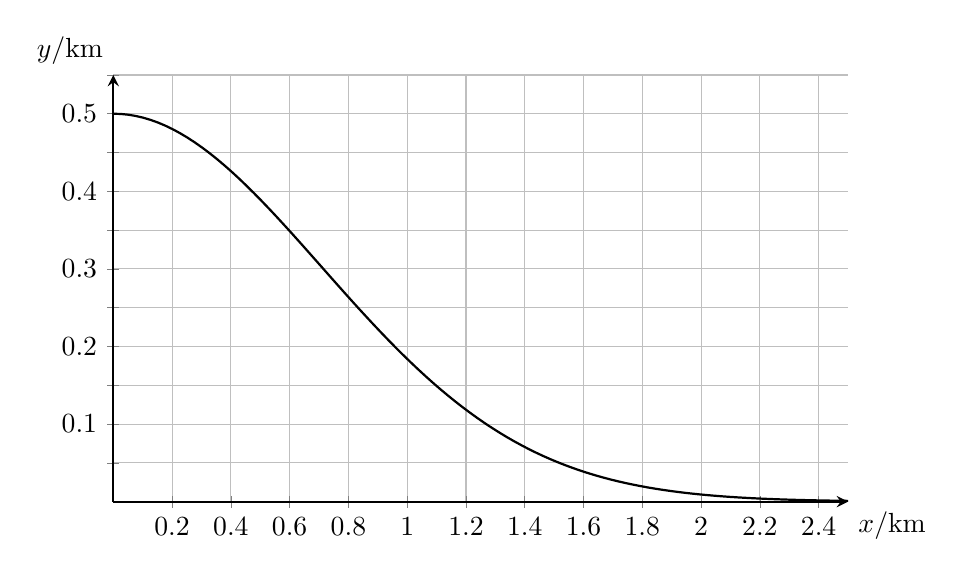
\begin{tikzpicture}
    \begin{axis}[               % indentering
        width=0.9\linewidth,    % indentering
        height=7cm,
        axis lines=middle,
        xlabel={$x$/km},
        ylabel={$y$/km},
        domain=0:2.5,
        samples=100,
        xmin=0,
        ymin=0,
        xmax=2.5,
        ymax=0.55,
        grid=major,
        thick,
        every axis x label/.style={
            at={(current axis.right of origin)}, anchor=north west},
        every  axis y label/.style={
            at={(current axis.above origin)}, anchor=south east},
        xtick={0,0.2,...,2.5},
        ytick={0,0.05,0.1,...,0.6},
        yticklabels={0.0,,0.1,,0.2,,0.3,,0.4,,0.5,,0.6}
    ]
        \addplot[black] {0.5*exp(-x^2)};
    \end{axis}
\end{tikzpicture}\newline
The graph is drawn with a relation between y (the height in km.) and x (the 
length in km.), which can be written as:\\ % radbrytning
$y = 0.5e^{-x^2}$ $\>$ $\>$ where $\>$ $\>$ $0 \leq x \leq 2.5$\\ % radbrytning
\section{The angle of a slope}
\label{sec:uppg1}
First we solve:\\ % radbrytning
\begin{addmargin}[1em]{1em}
    Determine the angle at which the curve of the function is inclined at the % indentering
    point $x=0,8$.\\ % radbrytning
\end{addmargin}
To do this, we first need to calculate the derivative 
$\left(\frac{dy}{dx}\right)$ of the function, which will give us the slope of 
the tangent line at that point. From the slope, we can then calculate the 
angle using the arctangent function. Because the function involves an 
exponential expression, we will use the \textbf{chain rule}:
\subsection{Splitting the function}
The function $y=0,5e^{-x^2}$ can be viewed as a composition of two functions:
\begin{itemize}
    \item The outer function $f(u)=0,5e^u$, where $u=-x^2$. % indentering
    \item The inner function $g(x)=-x^2$.
\end{itemize}
According to the chain rule, the derivative of the composite function is:
\begin{displaymath}
    \frac{dy}{dx} = \frac{dy}{du} \cdot \frac{du}{dx} % indentering
\end{displaymath}
\subsection{Step~1: Derivative of the Outer Function}
First, we differentiate the outer function $y = 0,5e^u$ with respect to $u$. 
The derivative of $e^u$ with respect to $u$ is simply $e^u$, and since there 
is a constant 0,5 in front, we have:
\begin{equation}
    \frac{dy}{du} = 0,5e^u % indentering
\end{equation}
\subsection{Step~2: Derivative of the Inner Function}
Next, we differentiate the inner function $u = -x^2$ with respect to $x$ using 
the basic power rule differentiation:
\begin{equation}
    \frac{du}{dx} = \frac{d}{dx}\left(-x^2\right) = -2x % indentering
\end{equation}
\subsection{Step~3: Applying the Chain Rule}
Now, we apply the chain rule by multiplying the results from Step~1 and Step~2:
\begin{equation}
    \frac{dy}{dx} = \frac{dy}{du} \cdot \frac{du}{dx} % indentering
    = 0,5e^{-x^2} \cdot \left(-2x\right)
\end{equation}
And by simplifying this expression we get:
\begin{equation}
    \frac{dy}{dx} = -x \cdot e^{-x^2} % indentering
\end{equation}
Thus we have the derivative of $y$.
\subsection{Finding the Slope at $x = 0,8$}
Now that we have the general expression for the derivative, we can calculate 
the slope of the curve at the point $x$. Substituting $x = 0,8$ into the 
derivative as well as simplifying:
\begin{equation}
    \begin{split} % indentering
        y'(0,8) & = -0,8 \cdot e^{-\left(0,8\right)^2} \\ % radbrytning
                & = -0,8 \cdot e^{-\left(0,64\right)} \\ % justering
                & \approx -0,8 \cdot 0,5272 \approx -0,42
    \end{split}
\end{equation}
So the answer is that the slope of the tangent line at $x = 0,8$ is 
approximately $-0,42$.
\section{The Steepest Point}
\label{sec:uppg2}
Here our task is:\\
\begin{addmargin}[1em]{1em}
    Find an equation where the angle is the steepest using this function: % indentering
    \begin{displaymath}
        y = 0,5e^{-ax^2} % indentering
    \end{displaymath}
\end{addmargin}
Where $a$ is a constant and $x$ is in the range $0 \leq x \leq 2,5$. 
Curves are steepest where their second derivative is zero so we'll need to 
find the second derivative. But first, we need to calculate the first 
derivative $y'$.
\subsection{First Derivative}
Just like earlier we will make use of the \textbf{chain rule} 
for this, so, again:
\begin{itemize}
    \item The outer function is $f(u) = 0.5e^u$, where $u = -ax^2$ % indentering
    \item The inner function is $g(x) = -ax^2$.
\end{itemize}
The outer function's derivative with respect to $u$ is, once again, $e^u$, 
so we have:
\begin{equation}
    \frac{dy}{du} = 0,5e^u % indentering
\end{equation}
And the inner function's derivative with respect to $x$ using the power rule, 
we get:
\begin{equation}
    \begin{split} % indentering
      \frac{du}{dx} &= \frac{d}{dx}\left(-ax^2\right) \\ % radbrytning
                    &= -2ax % justering
    \end{split}
\end{equation}
Now we can apply the chain rule:
\begin{equation}
    \begin{split} % indentering
      \frac{dy}{dx} &= \frac{dy}{du} \cdot \frac{du}{dx} \\ % radbrytning
                    &= 0,5e^{-ax^2} \cdot \left(-2ax\right) % justering
    \end{split}
\end{equation}
Now that we have the first derivative, we can simplify it:
\begin{displaymath}
    \begin{split} % indentering
      y'  &= 0,5e^{-ax^2} \cdot \left(-2ax\right) \\ % radbrytning
          &= -ax \cdot e^{-ax^2} % justering
    \end{split}
\end{displaymath}
\subsection{Finding the Second Derivative}
Finally we can work toward finding the Second Derivative $\frac{d^2y}{dx^2}$. 
To do this we can use the \textbf{quotient rule} and, once again, 
the \textbf{chain rule}.
\subsection*{The Quotient Rule}
The quotient rule states:
\begin{displaymath}
    \frac{f\left(x\right)}{g\left(x\right)} = % indentering
    \frac{f\left(x\right) \cdot g'\left(x\right) - f'\left(x\right) 
    \cdot g\left(x\right)}{g\left(x\right)^2}
\end{displaymath}
And in our case:
\begin{itemize}
    \item $f\left(x\right) = -ax$ % indentering
    \item $g\left(x\right) = e^{-ax^2}$
    \item $f'\left(x\right) = -a$
    \item $g'\left(x\right) = e^{ax^2} \cdot \left(2ax\right)$
\end{itemize}
So we can use this by rewriting the first derivative to make it suitable for 
the quotient rule:
\begin{displaymath}
    y' = \frac{-ax}{e^{ax^2}}
\end{displaymath}
Then we end up with:
\begin{equation}
    \begin{split} % indentering
        y'' &= \frac{\left(-a \cdot e^{ax^2}\right) - 
        \left(-ax\left(2ax \cdot e^{ax^2}\right)\right)}
        {\left(e^{ax^2}\right)^2} \\ % radbrytning
            &= \frac{-ae^{ax^2} + 2a^2x^2e^{ax^2}} % justering
            {\left(e^{ax^2}\right)^2}
    \end{split}
\end{equation}
Now if we factor out and have it equal $0$:
\begin{equation}
    \frac{ae^{ax^2}\left(-1+2ax^2\right)}
    {\left(e^{ax^2}\right)^2} = 0 % indentering
\end{equation}
Since this is division, only the numerator can be $0$, 
otherwise we would be dividing by $0$. 
So then that lets us solve where the curve is steepest:
\begin{displaymath}
    \begin{split} % indentering
        2ax^2-1 = 0 &\Rightarrow 1 = 2ax^2 \\ % radbrytning
                    &\Rightarrow x^2 = \frac{1}{2a} \\ % justering
                    &\Rightarrow x = \sqrt{\frac{1}{2a}}
    \end{split}
\end{displaymath}
\section{Pick Constant for Steepest Angle}
\label{sec:uppgN}
This task reads:\\ % radbrytning
\begin{addmargin}[1em]{1em}
    Pick a constant for $a$ which turns the slope in a way that % indentering
    turns the steepest angle to be at point $x = 1,0$
\end{addmargin}
We can make use of the work we did in the last task where we found
\begin{displaymath}
    x = \sqrt{\frac{1}{2a}} % indentering
\end{displaymath}
and by backtracking one step we can find the constant $a$ where $x = \pm 1$:
\begin{equation}
    \begin{split} % indentering
        x = \sqrt{\frac{1}{2a}} &\Rightarrow x^2 = \frac{1}{2a} \\% radbrytning
                                &\Rightarrow a = \frac{1}{2x^2} \\% justering
                                &\Rightarrow a = \frac{1}{2} = 0,5
    \end{split}
\end{equation}
\section{Conclusion}
\label{sec:disk}
The document effectively demonstrates how differentiation techniques, 
including the chain rule and quotient rule, are used to solve problems 
related to the slope and steepness of an exponential function. 
By calculating the derivative, it identifies the slope 
at a specific point and locates the steepest point on the curve. 
The selection of an appropriate constant shows how parameters can be 
adjusted to fit certain criteria, such as positioning the steepest 
point at a desired location. This approach highlights the practical 
application of calculus in analyzing the behavior of curves.
\subsection*{Results}
\begin{enumerate}
    \item \textbf{Slope at $x = 0.8$}: \\ % indentering & radbrytning
    After calculating the derivative $y'\left(x\right) = -x \cdot e^{-x^2}$,
    substituting $x=0.8$, the slope of the curve at that point is approximately
    $-0.42$. This indicates that the curve is decreasing at this point,
    with a relatively moderate rate of decline.
    \item \textbf{Steepest Point}: \\ % radbrytning
    By solving the second derivative $y''\left(x\right) = 0$, the curve is
    found to be steepest at $x = \sqrt{\frac{1}{2a}}$. This shows that the
    steepest point is influenced by the parameter $a$, and the steepness occurs
    closer to the origin as $a$ increases.
    \item \textbf{Determining the Constant $a$}: \\ % radbrytning
    To ensure the steepest point occurs at $x = 1,0$, the constant $a$ is
    calculated to be $0,5$. This result reflects the importance of parameter
    tuning in mathematical models and highlights how the shape of the function
    can be controlled by varying $a$.
\end{enumerate}
%
\begin{thebibliography}{99}
%
\bibitem{latexcompanion} 
Michel Goossens, Frank Mittelbach, and Alexander Samarin. 
\textit{The \LaTeX\ Companion}. 
Addison-Wesley, Reading, Massachusetts, 1993.
%
\bibitem{einstein} 
Albert Einstein. 
\textit{Zur Elektrodynamik bewegter K{\"o}rper}. (German) 
[\textit{On the electrodynamics of moving bodies}]. 
Annalen der Physik, 322(10):891–921, 1905.
%
\end{thebibliography}
%
\end{document}
